%!TEX root = ../main.tex
\section{Overview}
This chapter provides various tools and techniques that are used in this thesis like VLSW protocol used, SSIM model used and other language and framework details and platform used for realisation of the techniques proposed by this thesis.

\section{VLSW Protocol}
Variable-length sliding window protocol is a technique to generate time-series data for training machine learning or deep learning model. In this technique, a window of variable length is moved over the data, with zero-padding the remaining unaddressed bits of the window. For time series imputation of five consecutive timestamps, the variable-length window before and after that timestamp is collected and stacked into an array of data, and the actual values of that five timestamp data are used as the output of the algorithm. Figure \ref{fig:vlsw} describes the working of variable length sliding window protocol.

\begin{figure}[ht]
	\centering
	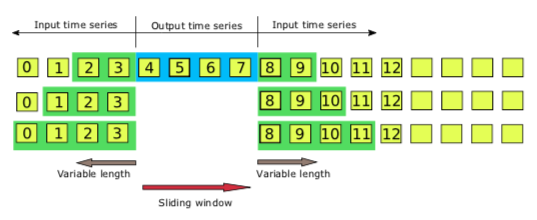
\includegraphics[width=0.8\textwidth]{images/vlsw.png}
	\caption{VLSW Protocol}
	\label{fig:vlsw}
\end{figure}

\section{Sequence to Sequence Imputation Model}
SSIM model module consist of 4 processes which are:
\begin{itemize}
\item Encoder
\item Attention layer
\item Decoder
\item Dense layer
\end{itemize}

\begin{figure}[ht]
	\centering
	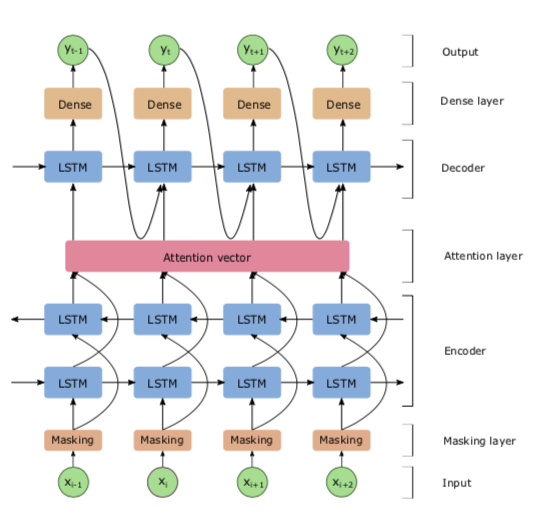
\includegraphics[width=0.5\textwidth]{images/ssim.png}
	\caption{SSIM Model Architecture}
	\label{fig:ssim}
\end{figure}

BiLSTM is used as the encoder which processes the data sequence in both directions i.e in forward direction and in backward direction. It checks for the pattern and learns its attention mechanism that  is used to focus on a specific part of the sequence which is necessary to generate the output sequence. Figure. \ref{fig:ssim} describes the SSIM model architecture.


\section{Implementation Tools}
Following is the disscussion about the tools that are used for implementing the models and training and testing the approach.

\subsection{Python}
Python is an interpreted, high-level, general-purpose programming language. It is widely used for programming machine, and deep learning algorithms, many famous machine learning, and deep learning libraries are built into python. Data scientists and data analysts widely use them. Prototyping is very easy in this language, and it is easy to learn and master. It is best suited for training deep learning models. The very famous deep learning framework Tensorflow is built using this language.

\subsection{Scikit Learn}
Scikit learn is a free opensource machine learning library written in python language. There may machine learning algorithms are implemented into this library like classification, regression, and clustering algorithms, including support vector machines, random forests, gradient boosting, k-means, and DBSCAN, and is designed to interoperate with the Python numerical and scientific libraries NumPy and SciPy. There are many helper functions and machine learning useful methods are implemented that can be used out of the box.

\subsection{Tensorflow}
Tensorflow is a software application popular for implementing machine learning algorithms, particularly neural networks. It was developed by Google it was released as an open-source platform in 2015. It is called Tensorflow because it takes input as a multidimensional array. Multidimensional arrays are also known as tensors you can construct a sort of flow chart of operation you want to perform on that input so input goes in at one end, and then it flows through this system of operation and comes out the other end as output, and that is why it is called TensorFlow. It's extremely versatile; it can be run on many diff platforms (computers, pc, laptops, raspberry pi, etc.). It can be trained on multiple machines. It can also run on GPU as well as CPU. There is tensorboard to help monitor the operation of machine learning algorithms visually.  

\subsection{Pandas}
Pandas is a python library that gives a great set of tools for data analysis. With pandas you can load prepare manipulate model and analyze data, can join data, reshape data, merge data, Combine datasets. It is very useful library for data manipulation. In this thesis the pandas is used to wrangel the dataset remove missing values and padding and careing the timestamps so that can be made in sequence manner so that deep learning algorithms can be applied to it.
\\

\subsection{Matplotlib}
Matplotlib is a tool for data visualization in python strongly coherred with numpy and pandas. It helped in the thesis for generating the result graphs and other graphs needed for the analysis.
\\

\subsection{Google Colab}
Google Colab is a Jupyter notebook in the google cloud pre installed with many machine learning and deep learning libraries generally needed for the data analysis data visualization, machine learning and deep learning. Beside that other not installed libraries can also be installed and used. It also provide the GPU (Graphics Processing Unit) support for training the models very fast as compared to CPU (Centeral Processing Unit) which is also available and can be used. Along with CPU and GPUs it comes with TPU (Tensor Processing Unit) which are special kind of GPU specialy designed to work with the very famous tensorflow framework. Currently it is only available in the google cloud hosted platforms like colab or for custom google compute cloud one can easily build and run machine learning algorithms in the cloud.
\\

\section{Summary}
In this chapter various tools and techniques are described that uare used for the development of the proposed work. The next chapter describes the solution to the problem using the tools and techniques.